\documentclass[12pt,letterpaper]{article}
\usepackage{fullpage}
\usepackage[top=2cm, bottom=4.5cm, left=2.5cm, right=2.5cm]{geometry}
\usepackage{amsmath,amsthm,amsfonts,amssymb,amscd}
\usepackage{lastpage}
\usepackage{enumerate}
\usepackage{fancyhdr}
\usepackage{mathrsfs}
\usepackage{xcolor}
\usepackage{graphicx}
\usepackage{listings}
\usepackage{hyperref}
\usepackage{tikz}
\usepackage{tikz-3dplot}
\usepackage{relsize}
\usepackage{fancyvrb}
\usetikzlibrary{shapes.geometric,fit}

\hypersetup{%
  colorlinks=true,
  linkcolor=blue,
  linkbordercolor={0 0 1}
}

\setlength{\parindent}{0.0in}
\setlength{\parskip}{0.05in}

\newcommand\course{MATH 1208}
\newcommand\hwnumber{11}
\newcommand\NetIDa{dc3451}
\newcommand\NetIDb{David Chen}

\theoremstyle{definition}
\newtheorem*{statement}{Statement}
\newtheorem*{claim}{Claim}
\newtheorem*{theorem}{Theorem}
\newtheorem*{lemma}{Lemma}

\newcommand{\contra}{\Rightarrow\!\Leftarrow}
\newcommand{\R}{\mathbb{R}}
\newcommand{\F}{\mathbb{F}}
\newcommand{\Z}{\mathbb{Z}}
\newcommand{\Zeq}{\mathbb{Z}_{\geq 0}}
\newcommand{\Zg}{\mathbb{Z}_{>0}}
\newcommand{\Req}{\mathbb{R}_{\geq 0}}
\newcommand{\Rg}{\mathbb{R}_{>0}}
\newcommand{\N}{\mathbb{N}}
\newcommand{\Q}{\mathbb{Q}}
\newcommand{\C}{\mathbb{C}}
\newcommand{\id}{\mathrm{Id}}
\newcommand{\im}{\mathrm{im}}
\newcommand{\tr}{\mathrm{tr}}
\newcommand{\diag}{\mathrm{diag}}
\newcommand{\rank}{\mathrm{rank}}
\newcommand{\spn}{\mathrm{span}}

\pagestyle{fancyplain}
\headheight 35pt
\lhead{\NetIDa}
\lhead{\NetIDa\\\NetIDb}
\chead{\textbf{\Large Homework \hwnumber}}
\rhead{\course \\ \today}
\lfoot{}
\cfoot{}
\rfoot{\small\thepage}
\headsep 1.5em

\begin{document}

\subsection*{Apostol p.362 no.1}

\begin{align*}
  \int_0^1\int_0^1xy(x+y)dydx &= \int_0^1\int_0^1(x^2y + xy^2)dydx \\
                              &= \int_0^1\left[ \frac{1}{2}x^2y^2 + \frac{1}{3}xy^3 \right]\Big|_{y=0}^{y=1}dx \\
                              &= \int_0^1 (\frac{1}{2}x^2 + \frac{1}{3}x)dx \\
                              &= \left[ \frac{1}{6}{x^3 + \frac{1}{6}x^2} \right]\Big|_{x=0}^{x=1} \\
                              &= \frac{1}{3}
\end{align*}

\subsection*{Apostol p.362 no.9}

\begin{claim}
  If $Q = [a_1,b_1] \times [a_2,b_2]$ is a rectangle and all of $\iint_Q fg,
  \int f, \int g$ exist, then
  \[
    \iint\limits_Q f(x)g(y)dxdy = \left( \int f(x)dx \right)\left( \int g(y)dy \right)
  \]
\end{claim}

\begin{proof}
  Put 
  \[
    \int_{a_1}^{b_1}f(x)dx = F, \int_{a_2}^{b_2}g(y)dy = G
  \]
  First, note that
  \[
    \int_{a_1}^{b_1}f(x)g(y)dx = g(y)\int_{a_1}^{b_1}f(x)dx = F \cdot g(y)
  \]
  
  \begin{align*}
    \iint\limits_Q f(x)g(y)dxdy &= \int_{a_2}^{b_2}\int_{a_1}^{b_1}f(x)g(y)dxdy \\
                                &= \int_{a_2}^{b_2} Fg(y)dy \\
                                &= F\int_{a_2}^{b_2}g(y)dy \\
                                &= FG
  \end{align*}
\end{proof}

\subsection*{Apostol p.363 no.14}

\begin{claim}
  Let $f:  Q \rightarrow \R$ where $Q = [0,1]\times[0,1]$ be given by
  \[
    f(x,y) =
    \begin{cases}
      1 & x = y \\
      0 & x \neq y
    \end{cases}
  \]

  Then, $\iint_Qf = 0$.
\end{claim}

\begin{proof}
  To show that the integral exists, for any $\epsilon > 0$, let $\epsilon' =
  \frac{p}{q}$ where $p, q \in \Zg$ be $0 < \epsilon' < \epsilon$. Now, consider
  a partition of $Q$ into $q^2$ subrectangles, where $R_{i,j} = [\frac{i-1}{q}, \frac{i}{q}]
  \times [\frac{j-1}{q}, \frac{j}{q}]$ where $1 \leq i,j \leq q$. Then, let
  \[
    s(x,y) = 0 \text{ and }
    t(x,y) =
    \begin{cases}
      1 & (x,y) \in R_{i,j}, i = j \\
      0 & \text{otherwise}
    \end{cases}
  \]
  Note that if $x = y$, then $(x,y) \in \R_{c,c}$ where $c = \lfloor xq \rfloor
  = \lfloor yq \rfloor$. Then, we have that $s \leq f \leq t$, and that
  \[
    \iint\limits_Q (t-s) = \iint\limits_Qt = \frac{1}{q^2} = \frac{1}{q} <
    \frac{p}{q} = \epsilon' = \epsilon
  \]

  Thus, the integral exists; further, we have that $\iint_Q s = 0, \iint_Q t <
  \epsilon$ for any $\epsilon > 0$ which yields that
  \[
    \iint\limits_Q s \leq \iint\limits_Qf \leq \iint\limits_Qt \implies 0 \leq
    \iint\limits_Qf \leq \epsilon \implies \iint\limits_Qf = 0
  \]
\end{proof}

\subsection*{Apostol p.372 no.1}

For drawings, see attached picture at end.

\begin{align*}
  \iint\limits_Sx\cos(x+y)dxdy &= \int_0^\pi\int_0^xx\cos(x+y)dydx \\
                               &= \int_0^\pi\left[ -x\sin(x+y) \right]\Big|_{y=0}^{y=x}dx \\
                               &= \int_0^\pi x(\sin(x)-\sin(2x))dx \\
                               &= \left[ -x\cos(x) + \frac{1}{2}x\cos(x) + \sin(x) - \frac{1}{4}\sin(2x) \right]\Big|_{x=0}^{x=\pi} \\
                               &= \frac{3\pi}{2}
\end{align*}

\subsection*{Apostol p.372 no.7}

\begin{align*}
  \int_{1}^{3}\int_{-x}^x(x^2-y^2)dydx &= \int_1^3\left[ x^2y - \frac{1}{3}y^3 \right]\Big|_{y=-x}^{y=x}dx \\
                                       &= \int_1^3 \frac{4}{3}x^3dx \\
                                       &= \left[ \frac{1}{4}x^4 \right]\Big|_{x=1}^{x=3} \\
                                       &= \frac{80}{3} 
\end{align*}

\subsection*{Apostol p.372 no.14}

\[
  \int_0^1\int_0^{\log{x}}f(x,y)dydx = \int_0^1\int_{e^y}^ef(x,y)dxdy
\]

\section*{Problem 1}

Fix $\epsilon > 0$, and suppose that $\exists \delta > 0 \mid |x - y| < \delta
\implies |g(x,t) - g(y,t)| < \epsilon$ for all $t \in (0,1)$. Consider $t = 1 -
\frac{\delta}{4\epsilon}$ and $y = x + \frac{\delta}{2}$. Then,
\[
  \left|g(x,t) - g(y,t)\right| = \left|\frac{x}{1-t} - \frac{y}{1-t}\right| =
  \frac{4\frac{\delta}{2}}{\delta}\epsilon = 2\epsilon > \epsilon
\]

This gives $\contra$, so the lemma on uniform continuity needs not hold on open $Q$.

\section*{Problem 2}

\subsubsection*{a}

\begin{claim}
  \[
    f(x,y) = \chi_{\Q}(xy)
    % \begin{cases}
    %   1 & xy \in \Q \\
    %   0 & xy \notin \Q
    % \end{cases}
  \]
  where $\chi_\Q$ is the indicator function on $\Q$,
  is not (Riemann) integrable on $S = [0,1] \times [0,1]$. 
\end{claim}

\begin{proof}
  Consider any step function $s \leq f$. Suppose that $s > 0$ on some
  subrectangle $R = [x,x + \epsilon_1] \times [y,y + \epsilon_2] \subset S$.
  Then, from the density of the irrationals in $\R$, we have that $\exists x', y'
  \notin \Q \mid x < x' < x + \epsilon_1$ and $y < y' < y + \epsilon_2$. Then,
  $f(x',y') = 0$ and so $s(x',y') > f(x',y')$.

  Similarly, for any step function $t \geq f$, suppose $t < 1$ on some
  subrectangle $R = [x,x + \epsilon_1] \times [y,y + \epsilon_2] \subset S$.
  Then, from the density of $\Q$ in $\R$, we have that $\exists x', y'
  \in \Q \mid x < x' < x + \epsilon_1$ and $y < y' < y + \epsilon_2$. Then,
  $f(x',y') = 1$ and so $t(x',y') < f(x',y')$.

  Thus, from the comparison theorem $\int_S s \leq \int_S 0 = 0$, and $\int_S t
  \geq \int_S 1 = 1$, such that $\underline{I}(f) = 0 \neq \overline{I}(f) = 1$.
  Thus, $f$ is not integrable.
\end{proof}

\subsubsection*{b}

\begin{claim}
  \[
    g(x,y) =
    \begin{cases}
      0 & y < \frac{1}{2}, y > \frac{1}{2} \\
      \chi_\Q(x) & y = \frac{1}{2}
    \end{cases}
  \]
  where $\chi_\Q$ is the indicator function on $\Q$,
  has that $\int_0^1g(x,y)dy$ exists for any fixed $x$, but $\int_0^1g(x,y)dx$
  does not for $y = \frac{1}{2}$.
\end{claim}

\begin{proof}
  \[
    \int_0^1g(x,\frac{1}{2})dx = \int_0^1\chi_\Q(x)
  \]
  which is not integrable as shown in the first semester.

  For $\int_0^1g(x,y)dy$, we can directly compute the integral to be 0; for any
  $\epsilon > 0$, consider that we can get the step functions
  \[
    s(y) =
    \begin{cases}
      -\frac{\epsilon}{3} & y < \frac{1}{2}, y > \frac{1}{2} \\
      0 & y = \frac{1}{2}
    \end{cases} \text{ and }
    t(y) =
    \begin{cases}
      \frac{\epsilon}{3} & y < \frac{1}{2}, y > \frac{1}{2} \\
      1 & y = \frac{1}{2}
    \end{cases}
  \]
  such that $s \leq f \leq t$. Then, we have that 
  \[
    \int (t - s) = \frac{2\epsilon}{3} < \epsilon
  \]
  which implies that $f$ is integrable.
  % \[
  %   \int s \leq \int f \leq \int t \implies -\frac{\epsilon}{3} \leq \int f \leq \frac{\epsilon}{3}
  %   \implies \left|\int f\right| \leq \frac{\epsilon}{3} \implies \left|\int f\right| = 0
  % \]
\end{proof}

\subsubsection*{c}

\begin{claim}
  \[
    h(x,y) = \chi_\Q(x)
  \]
  where $\chi_\Q$ is the indicator function on $\Q$,
  has that $\int_0^1h(x,y)dy$ exists for any fixed $x$, but
  $\int_0^1\int_0^1h(x,y)dxdy$ does not exist.
\end{claim}

\begin{proof}
  Note that
  \[
    \int_0^1h(x,y)dy =
    \begin{cases}
      \int_0^1 1 dy & x \in \Q \\
      \int_0^1 0 dy & x \notin \Q
    \end{cases} =
    \begin{cases}
      1 & x \in \Q \\
      0 & x \notin \Q
    \end{cases} = \chi_\Q(x)
  \] 

  So the integral $\int_0^1h(x,y)dy$ exists. 
  $\int_0^1\int_0^1h(x,y)dxdy$ does not exist by reasoning similar to part a of
  this question.

  Consider any step function $s \leq h$. Suppose that $s > 0$ on some
  subrectangle $R = [x,x + \epsilon_1] \times [y,y + \epsilon_2] \subset S$.
  Then, from the density of the irrationals in $\R$, we have that $\exists x'
  \notin \Q \mid x < x' < x + \epsilon_2$. Then,
  $h(x',y + \frac{\epsilon_2}{2}) = 0$ and so $s(x',y + \frac{\epsilon_2}{2}) >
  h(x',y + \frac{\epsilon_2}{2})$.

  Similarly, for any step function $t \geq h$, suppose $t < 1$ on some
  subrectangle $R = [x,x + \epsilon_1] \times [y,y + \epsilon_2] \subset S$.
  Then, from the density of $\Q$ in $\R$, we have that $\exists x'
  \in \Q \mid x < x' < x + \epsilon_1$ Then,
  $h(x',y + \frac{\epsilon_2}{2}) = 1$ and so $t(x',y + \frac{\epsilon_2}{2}) < h(x',y + \frac{\epsilon_2}{2})$.

  Thus, from the comparison theorem $\int_S s \leq \int_S 0 = 0$, and $\int_S t
  \geq \int_S 1 = 1$, such that $\underline{I}(f) = 0 \neq \overline{I}(f) = 1$.
  Thus, $f$ is not integrable.
\end{proof}

\section*{Problem 4}

\subsection*{a}

\begin{claim}
  For $S, T$ disjoint bounded subsets of $\R^n$ and $f: \R^n \rightarrow \R$, if
  $\int_Sf$ and $\int_T f$ exist, then $\int_{S \cup T}f = \int_Sf + \int_Tf$.
\end{claim}

\begin{proof}
  Let $S \subset Q_S, T \subset Q_T$ where $Q_S,Q_T$ are closed rectangles.
  Then, if $Q_S = [a_1, b_1] \times \cdots \times [a_n,b_n]$ and $Q_T =
  [c_1,d_1] \times \cdots \times [c_n,d_n],$ consider
  \[Q =
    [\min\{a_1,c_1\},\max\{b_1,d_1\}] \times \cdots
    [\min\{a_b,c_b\},\max\{b_b,d_b\}]
  \] Then, $Q$ is a closed rectangle such that
  $Q_s, Q_T \subset Q$.

  Now consider the extension by zero functions $f_S, f_T, f_U: Q \rightarrow \R$.
  \begin{align*}
    f_S(x) &=
             \begin{cases}
               f(x) & x \in S \\
               0 & \text{otherwise}
             \end{cases} \\
    f_T(x) &=
             \begin{cases}
               f(x) & x \in T \\
               0 & \text{otherwise}
             \end{cases} \\
    f_U(x) &=
             \begin{cases}
               f(x) & x \in S \cup T \\
               0 & \text{otherwise}
             \end{cases}
  \end{align*}

  Then by definition, $\int_Sf = \int_Qf_S$, $\int_Tf = \int_Qf_T, \int_{S\cup T}f =
  \int_Qf_U$.

  Note that
  \[
    f_S(x) + f_T(x) =
    \begin{cases}
      f_S(x) + f_T(x) & x \in S \\
      f_S(x) + f_T(x) & x \in T \\
      f_S(x) + f_T(x) & \text{otherwise}
    \end{cases} = 
    \begin{cases}
      f(x) + 0 & x \in S \\
      0 + f(x) & x \in T \\
      0 + 0 & \text{otherwise}
    \end{cases}
    = f_U(x)
  \]
  as $S, T$ are disjoint. Then, additivity of the integral yields $\int_Q(f_S + f_T) = \int_Q(f_U)$, which gives
  us the desired result.
\end{proof}

\subsection*{b}

\begin{claim}
  For $S, T$ bounded subsets of $\R^n$ which intersect in a hyperplane $x_i = c$ and $f: \R^n \rightarrow \R$, if
  $\int_Sf$ and $\int_T f$ exist, then $\int_{S \cup T}f = \int_Sf + \int_Tf$.
\end{claim}

\begin{proof}
  Take the same definition for $Q$ as above. We will prove that $\int_Qg = 0$
  where
  \[
    g(x) =
    \begin{cases}
      f(x) & x \in S \cap T \\
      0 & \text{otherwise}
    \end{cases}
  \]
  where $S \cap T$ is a subset of the hyperplane $x_i = c$.
  
  Consider $s \leq g \leq t$ where $s, t$ are step functions $Q \rightarrow \R$.

  Then, $s \leq 0$. Consider any subrectangle $R = [a_1, b_1]
  \times \cdots \times [a_n, b_n]$. In particular, if $c \notin [a_i, b_i]$,
  then we have that $f = 0$ on $R$; if $c \in [a_i, b_i]$, then $x =
  (\frac{a_1+b_1}{2}, \frac{a_2+b_2}{2} , \dots, c + \epsilon, \dots,
  \frac{a_{n-1}+b_{n-1}}{2}, \frac{a_n+b_n}{2}) \in R$, where $c + \epsilon \in
  [a_i, b_i], \epsilon \neq 0$ and we have that $f(x) =
  0, s(x) \leq 0$ and thus $s \leq 0$ on any subrectangle $R$.

  Further, $t \leq 0$. Consider any subrectangle $R = [a_1, b_1]
  \times \cdots \times [a_n, b_n]$. In particular, if $c \notin [a_i, b_i]$,
  then we have that $f = 0$ on $R$; if $c \in [a_i, b_i]$, then $x =
  (\frac{a_1+b_1}{2}, \frac{a_2+b_2}{2} , \dots, c + \epsilon, \dots,
  \frac{a_{n-1}+b_{n-1}}{2}, \frac{a_n+b_n}{2}) \in R$ where $c + \epsilon \in
  [a_i, b_i], \epsilon \neq 0$, and we have that $f(x) =
  0, t(x) \geq 0$ and thus $t \geq 0$ on any subrectangle $R$.

  We give now $s, t$ such that $\int_Q s = \int_Qt = 0$. If $f$ is bounded by
  $K$ on $Q$,
  \[
    Q = [a_1, b_1] \times \cdots \times [a_n,b_n]
  \]
  define
  \[
    Q_s = [a_1, b_i] \times \cdots \times [a_i, c] \times \dots [a_n, b_n]
  \]
  \[
    Q_t = [a_1, b_i] \times \cdots \times [c,b_i] \times \dots [a_n, b_n]
  \]
  and
  \begin{gather*}
    s =
    \begin{cases}
      0 & x \in Q_s \\
      0 & x \in Q_t \\
      -K & x_i = c
    \end{cases} \\
    t = 
    \begin{cases}
      0 & x \in Q_s \\
      0 & x \in Q_t \\
      K & x_i = c
    \end{cases}
  \end{gather*}

  Then, we have that $\underline{I}(g) = \overline{I}(g) = 0$.
  
  Take the same definitions for $Q, f_S, f_T, f_U$ as part a. Then, we have that
  $f_S + f_T - g = f_U$, which then gives that
  \[
    \int_Q(f_S + f_T - g) = \int_Qf_S +  \int_Qf_T - 0 = \int_Qf_U \implies \int_Sf + \int_Tf = \int_{S\cup T}f
  \]
\end{proof}

\begin{center}
  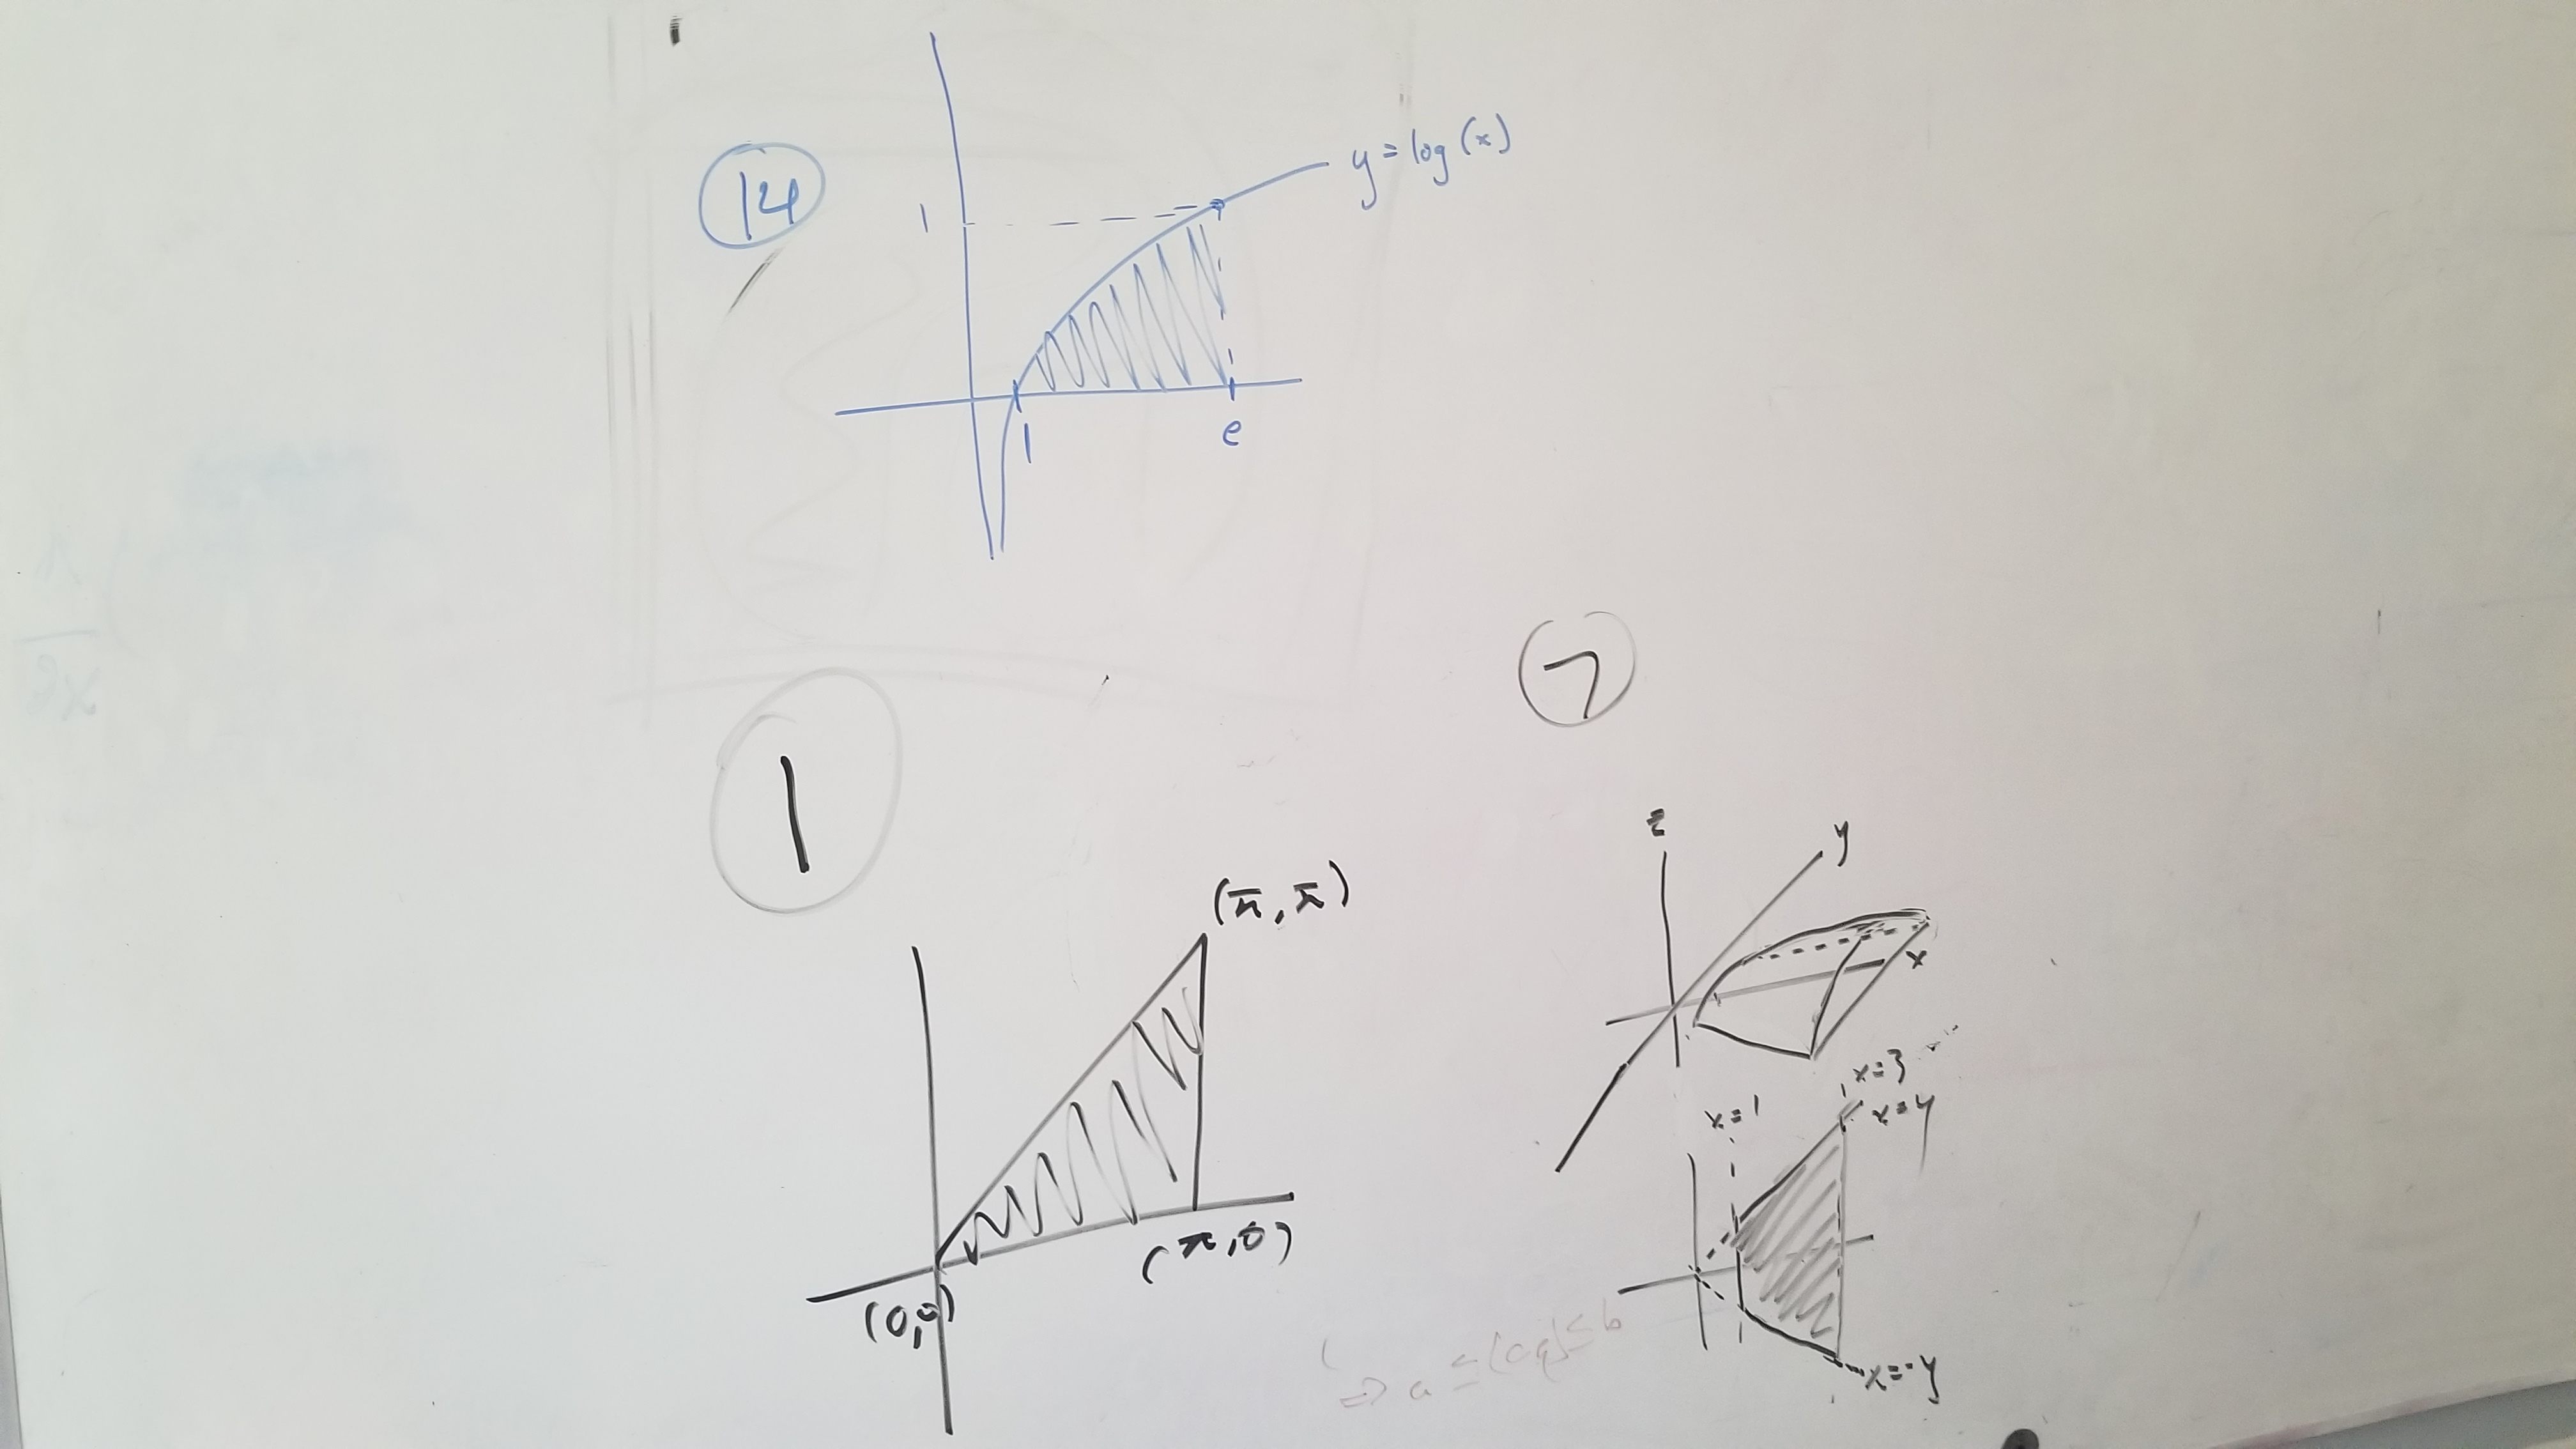
\includegraphics[height=3.5in]{./domains.jpg}
\end{center}

\end{document}

% LocalWords:  NetID fancyplain LocalWords colorlinks linkcolor linkbordercolor
% LocalWords:  Apostol
 